% Options for packages loaded elsewhere
\PassOptionsToPackage{unicode}{hyperref}
\PassOptionsToPackage{hyphens}{url}
\PassOptionsToPackage{dvipsnames,svgnames,x11names}{xcolor}
%
\documentclass[
  letterpaper,
  DIV=11,
  numbers=noendperiod]{scrartcl}

\usepackage{amsmath,amssymb}
\usepackage{lmodern}
\usepackage{iftex}
\ifPDFTeX
  \usepackage[T1]{fontenc}
  \usepackage[utf8]{inputenc}
  \usepackage{textcomp} % provide euro and other symbols
\else % if luatex or xetex
  \usepackage{unicode-math}
  \defaultfontfeatures{Scale=MatchLowercase}
  \defaultfontfeatures[\rmfamily]{Ligatures=TeX,Scale=1}
\fi
% Use upquote if available, for straight quotes in verbatim environments
\IfFileExists{upquote.sty}{\usepackage{upquote}}{}
\IfFileExists{microtype.sty}{% use microtype if available
  \usepackage[]{microtype}
  \UseMicrotypeSet[protrusion]{basicmath} % disable protrusion for tt fonts
}{}
\makeatletter
\@ifundefined{KOMAClassName}{% if non-KOMA class
  \IfFileExists{parskip.sty}{%
    \usepackage{parskip}
  }{% else
    \setlength{\parindent}{0pt}
    \setlength{\parskip}{6pt plus 2pt minus 1pt}}
}{% if KOMA class
  \KOMAoptions{parskip=half}}
\makeatother
\usepackage{xcolor}
\setlength{\emergencystretch}{3em} % prevent overfull lines
\setcounter{secnumdepth}{-\maxdimen} % remove section numbering
% Make \paragraph and \subparagraph free-standing
\ifx\paragraph\undefined\else
  \let\oldparagraph\paragraph
  \renewcommand{\paragraph}[1]{\oldparagraph{#1}\mbox{}}
\fi
\ifx\subparagraph\undefined\else
  \let\oldsubparagraph\subparagraph
  \renewcommand{\subparagraph}[1]{\oldsubparagraph{#1}\mbox{}}
\fi

\usepackage{color}
\usepackage{fancyvrb}
\newcommand{\VerbBar}{|}
\newcommand{\VERB}{\Verb[commandchars=\\\{\}]}
\DefineVerbatimEnvironment{Highlighting}{Verbatim}{commandchars=\\\{\}}
% Add ',fontsize=\small' for more characters per line
\usepackage{framed}
\definecolor{shadecolor}{RGB}{241,243,245}
\newenvironment{Shaded}{\begin{snugshade}}{\end{snugshade}}
\newcommand{\AlertTok}[1]{\textcolor[rgb]{0.68,0.00,0.00}{#1}}
\newcommand{\AnnotationTok}[1]{\textcolor[rgb]{0.37,0.37,0.37}{#1}}
\newcommand{\AttributeTok}[1]{\textcolor[rgb]{0.40,0.45,0.13}{#1}}
\newcommand{\BaseNTok}[1]{\textcolor[rgb]{0.68,0.00,0.00}{#1}}
\newcommand{\BuiltInTok}[1]{\textcolor[rgb]{0.00,0.23,0.31}{#1}}
\newcommand{\CharTok}[1]{\textcolor[rgb]{0.13,0.47,0.30}{#1}}
\newcommand{\CommentTok}[1]{\textcolor[rgb]{0.37,0.37,0.37}{#1}}
\newcommand{\CommentVarTok}[1]{\textcolor[rgb]{0.37,0.37,0.37}{\textit{#1}}}
\newcommand{\ConstantTok}[1]{\textcolor[rgb]{0.56,0.35,0.01}{#1}}
\newcommand{\ControlFlowTok}[1]{\textcolor[rgb]{0.00,0.23,0.31}{#1}}
\newcommand{\DataTypeTok}[1]{\textcolor[rgb]{0.68,0.00,0.00}{#1}}
\newcommand{\DecValTok}[1]{\textcolor[rgb]{0.68,0.00,0.00}{#1}}
\newcommand{\DocumentationTok}[1]{\textcolor[rgb]{0.37,0.37,0.37}{\textit{#1}}}
\newcommand{\ErrorTok}[1]{\textcolor[rgb]{0.68,0.00,0.00}{#1}}
\newcommand{\ExtensionTok}[1]{\textcolor[rgb]{0.00,0.23,0.31}{#1}}
\newcommand{\FloatTok}[1]{\textcolor[rgb]{0.68,0.00,0.00}{#1}}
\newcommand{\FunctionTok}[1]{\textcolor[rgb]{0.28,0.35,0.67}{#1}}
\newcommand{\ImportTok}[1]{\textcolor[rgb]{0.00,0.46,0.62}{#1}}
\newcommand{\InformationTok}[1]{\textcolor[rgb]{0.37,0.37,0.37}{#1}}
\newcommand{\KeywordTok}[1]{\textcolor[rgb]{0.00,0.23,0.31}{#1}}
\newcommand{\NormalTok}[1]{\textcolor[rgb]{0.00,0.23,0.31}{#1}}
\newcommand{\OperatorTok}[1]{\textcolor[rgb]{0.37,0.37,0.37}{#1}}
\newcommand{\OtherTok}[1]{\textcolor[rgb]{0.00,0.23,0.31}{#1}}
\newcommand{\PreprocessorTok}[1]{\textcolor[rgb]{0.68,0.00,0.00}{#1}}
\newcommand{\RegionMarkerTok}[1]{\textcolor[rgb]{0.00,0.23,0.31}{#1}}
\newcommand{\SpecialCharTok}[1]{\textcolor[rgb]{0.37,0.37,0.37}{#1}}
\newcommand{\SpecialStringTok}[1]{\textcolor[rgb]{0.13,0.47,0.30}{#1}}
\newcommand{\StringTok}[1]{\textcolor[rgb]{0.13,0.47,0.30}{#1}}
\newcommand{\VariableTok}[1]{\textcolor[rgb]{0.07,0.07,0.07}{#1}}
\newcommand{\VerbatimStringTok}[1]{\textcolor[rgb]{0.13,0.47,0.30}{#1}}
\newcommand{\WarningTok}[1]{\textcolor[rgb]{0.37,0.37,0.37}{\textit{#1}}}

\providecommand{\tightlist}{%
  \setlength{\itemsep}{0pt}\setlength{\parskip}{0pt}}\usepackage{longtable,booktabs,array}
\usepackage{calc} % for calculating minipage widths
% Correct order of tables after \paragraph or \subparagraph
\usepackage{etoolbox}
\makeatletter
\patchcmd\longtable{\par}{\if@noskipsec\mbox{}\fi\par}{}{}
\makeatother
% Allow footnotes in longtable head/foot
\IfFileExists{footnotehyper.sty}{\usepackage{footnotehyper}}{\usepackage{footnote}}
\makesavenoteenv{longtable}
\usepackage{graphicx}
\makeatletter
\def\maxwidth{\ifdim\Gin@nat@width>\linewidth\linewidth\else\Gin@nat@width\fi}
\def\maxheight{\ifdim\Gin@nat@height>\textheight\textheight\else\Gin@nat@height\fi}
\makeatother
% Scale images if necessary, so that they will not overflow the page
% margins by default, and it is still possible to overwrite the defaults
% using explicit options in \includegraphics[width, height, ...]{}
\setkeys{Gin}{width=\maxwidth,height=\maxheight,keepaspectratio}
% Set default figure placement to htbp
\makeatletter
\def\fps@figure{htbp}
\makeatother

\KOMAoption{captions}{tableheading}
\makeatletter
\makeatother
\makeatletter
\makeatother
\makeatletter
\@ifpackageloaded{caption}{}{\usepackage{caption}}
\AtBeginDocument{%
\ifdefined\contentsname
  \renewcommand*\contentsname{Table of contents}
\else
  \newcommand\contentsname{Table of contents}
\fi
\ifdefined\listfigurename
  \renewcommand*\listfigurename{List of Figures}
\else
  \newcommand\listfigurename{List of Figures}
\fi
\ifdefined\listtablename
  \renewcommand*\listtablename{List of Tables}
\else
  \newcommand\listtablename{List of Tables}
\fi
\ifdefined\figurename
  \renewcommand*\figurename{Figure}
\else
  \newcommand\figurename{Figure}
\fi
\ifdefined\tablename
  \renewcommand*\tablename{Table}
\else
  \newcommand\tablename{Table}
\fi
}
\@ifpackageloaded{float}{}{\usepackage{float}}
\floatstyle{ruled}
\@ifundefined{c@chapter}{\newfloat{codelisting}{h}{lop}}{\newfloat{codelisting}{h}{lop}[chapter]}
\floatname{codelisting}{Listing}
\newcommand*\listoflistings{\listof{codelisting}{List of Listings}}
\makeatother
\makeatletter
\@ifpackageloaded{caption}{}{\usepackage{caption}}
\@ifpackageloaded{subcaption}{}{\usepackage{subcaption}}
\makeatother
\makeatletter
\@ifpackageloaded{tcolorbox}{}{\usepackage[many]{tcolorbox}}
\makeatother
\makeatletter
\@ifundefined{shadecolor}{\definecolor{shadecolor}{rgb}{.97, .97, .97}}
\makeatother
\makeatletter
\makeatother
\ifLuaTeX
  \usepackage{selnolig}  % disable illegal ligatures
\fi
\IfFileExists{bookmark.sty}{\usepackage{bookmark}}{\usepackage{hyperref}}
\IfFileExists{xurl.sty}{\usepackage{xurl}}{} % add URL line breaks if available
\urlstyle{same} % disable monospaced font for URLs
\hypersetup{
  pdftitle={Class 7 : Clustering and PCA},
  pdfauthor={Ryan Chung PID A15848050},
  colorlinks=true,
  linkcolor={blue},
  filecolor={Maroon},
  citecolor={Blue},
  urlcolor={Blue},
  pdfcreator={LaTeX via pandoc}}

\title{Class 7 : Clustering and PCA}
\author{Ryan Chung PID A15848050}
\date{}

\begin{document}
\maketitle
\ifdefined\Shaded\renewenvironment{Shaded}{\begin{tcolorbox}[frame hidden, breakable, borderline west={3pt}{0pt}{shadecolor}, interior hidden, enhanced, sharp corners, boxrule=0pt]}{\end{tcolorbox}}\fi

\#Clustering First let's make up some data to cluster so we can get a
feel for these methods and how to work with them

We can use the \texttt{rnorm()} function to generate random numbers from
a normal distribution centered around \texttt{mean}

\begin{Shaded}
\begin{Highlighting}[]
\FunctionTok{hist}\NormalTok{(}\FunctionTok{rnorm}\NormalTok{(}\DecValTok{5000}\NormalTok{, }\AttributeTok{mean =} \DecValTok{3}\NormalTok{)) }\CommentTok{\#histogram/data centered around mean value}
\end{Highlighting}
\end{Shaded}

\begin{figure}[H]

{\centering 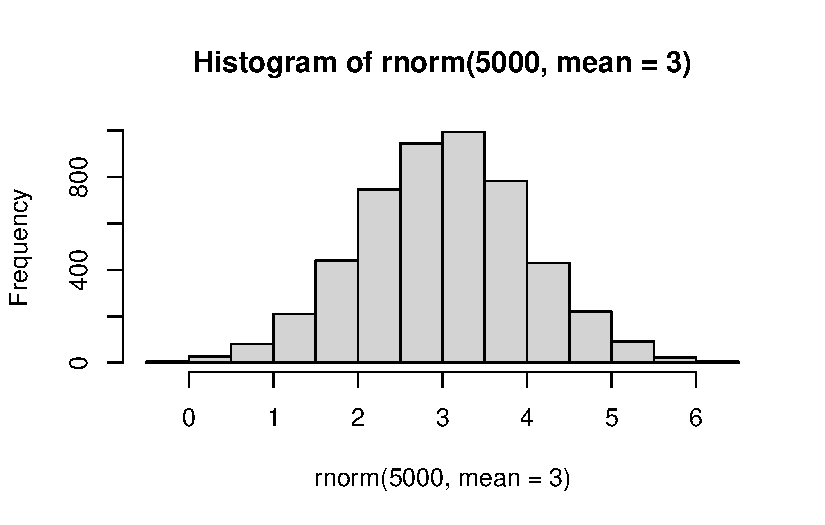
\includegraphics{Class07_files/figure-pdf/unnamed-chunk-1-1.pdf}

}

\end{figure}

Lets get 30 points with a mean of 3

\begin{Shaded}
\begin{Highlighting}[]
\NormalTok{test }\OtherTok{\textless{}{-}} \FunctionTok{c}\NormalTok{(}\FunctionTok{rnorm}\NormalTok{(}\DecValTok{30}\NormalTok{, }\AttributeTok{mean =} \DecValTok{3}\NormalTok{), }\FunctionTok{rnorm}\NormalTok{(}\DecValTok{30}\NormalTok{, }\AttributeTok{mean =} \SpecialCharTok{{-}}\DecValTok{3}\NormalTok{))}

\CommentTok{\#cbind,rev functions }
\end{Highlighting}
\end{Shaded}

\begin{Shaded}
\begin{Highlighting}[]
\NormalTok{x }\OtherTok{\textless{}{-}} \FunctionTok{cbind}\NormalTok{(}\AttributeTok{x =}\NormalTok{ test, }\AttributeTok{y =} \FunctionTok{rev}\NormalTok{(test))}

\FunctionTok{rev}\NormalTok{( (}\FunctionTok{c}\NormalTok{(}\DecValTok{1}\SpecialCharTok{:}\DecValTok{5}\NormalTok{)))}
\end{Highlighting}
\end{Shaded}

\begin{verbatim}
[1] 5 4 3 2 1
\end{verbatim}

\begin{Shaded}
\begin{Highlighting}[]
\FunctionTok{plot}\NormalTok{(x)}
\end{Highlighting}
\end{Shaded}

\begin{figure}[H]

{\centering 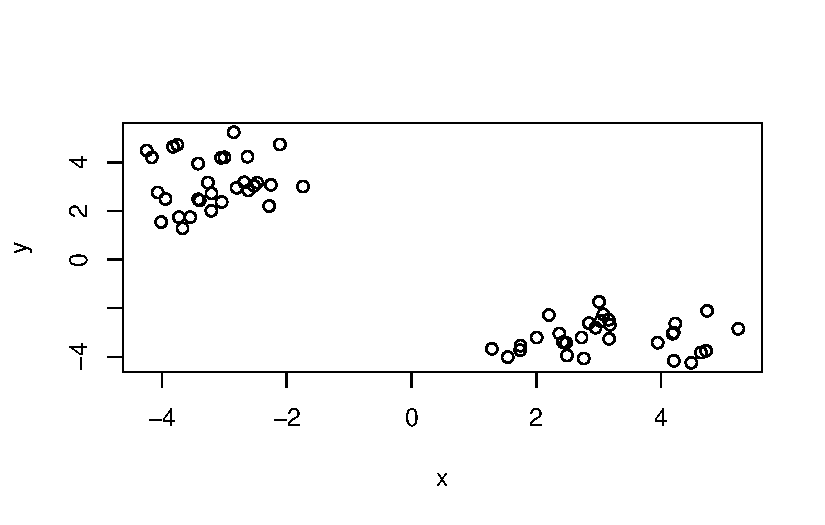
\includegraphics{Class07_files/figure-pdf/unnamed-chunk-3-1.pdf}

}

\end{figure}

\#\#K-means clustering

Very popular clustering method that we can use with the
\texttt{kmeans()} function in base R.

\begin{Shaded}
\begin{Highlighting}[]
\CommentTok{\#anything with an equal sign is not necessary ?}
\CommentTok{\#kmeans only needs an x, and centers arguement, centers {-} \# of clusters or \textquotesingle{}K\textquotesingle{}}

\NormalTok{km }\OtherTok{\textless{}{-}} \FunctionTok{kmeans}\NormalTok{(x, }\AttributeTok{centers =} \DecValTok{2}\NormalTok{)}
\NormalTok{km}
\end{Highlighting}
\end{Shaded}

\begin{verbatim}
K-means clustering with 2 clusters of sizes 30, 30

Cluster means:
          x         y
1 -3.164186  3.159142
2  3.159142 -3.164186

Clustering vector:
 [1] 2 2 2 2 2 2 2 2 2 2 2 2 2 2 2 2 2 2 2 2 2 2 2 2 2 2 2 2 2 2 1 1 1 1 1 1 1 1
[39] 1 1 1 1 1 1 1 1 1 1 1 1 1 1 1 1 1 1 1 1 1 1

Within cluster sum of squares by cluster:
[1] 45.91948 45.91948
 (between_SS / total_SS =  92.9 %)

Available components:

[1] "cluster"      "centers"      "totss"        "withinss"     "tot.withinss"
[6] "betweenss"    "size"         "iter"         "ifault"      
\end{verbatim}

\#\#\#kmean checkpoint questions \textgreater Q: Use the components to
find out- Cluster size, cluster membership, and center

\begin{Shaded}
\begin{Highlighting}[]
\NormalTok{km}\SpecialCharTok{$}\NormalTok{size }\CommentTok{\#Returns you cluster sizes {-} 30 points per cluster}
\end{Highlighting}
\end{Shaded}

\begin{verbatim}
[1] 30 30
\end{verbatim}

\begin{Shaded}
\begin{Highlighting}[]
\NormalTok{km}\SpecialCharTok{$}\NormalTok{cluster }\CommentTok{\#Returns cluster assignments}
\end{Highlighting}
\end{Shaded}

\begin{verbatim}
 [1] 2 2 2 2 2 2 2 2 2 2 2 2 2 2 2 2 2 2 2 2 2 2 2 2 2 2 2 2 2 2 1 1 1 1 1 1 1 1
[39] 1 1 1 1 1 1 1 1 1 1 1 1 1 1 1 1 1 1 1 1 1 1
\end{verbatim}

\begin{Shaded}
\begin{Highlighting}[]
\NormalTok{km}\SpecialCharTok{$}\NormalTok{centers }\CommentTok{\#Returns the coordinates of your centers }
\end{Highlighting}
\end{Shaded}

\begin{verbatim}
          x         y
1 -3.164186  3.159142
2  3.159142 -3.164186
\end{verbatim}

\begin{quote}
Q: Plot x, colored by means cluster assignment, adding cluster centers
as blue points
\end{quote}

\begin{Shaded}
\begin{Highlighting}[]
\NormalTok{mycols }\OtherTok{\textless{}{-}} \FunctionTok{c}\NormalTok{(km}\SpecialCharTok{$}\NormalTok{cluster)}
\FunctionTok{plot}\NormalTok{(x, }\AttributeTok{col =}\NormalTok{ mycols )}
\FunctionTok{points}\NormalTok{(km}\SpecialCharTok{$}\NormalTok{centers, }\AttributeTok{col =} \StringTok{"blue"}\NormalTok{, }\AttributeTok{pch =} \DecValTok{15}\NormalTok{ , }\AttributeTok{cex =} \DecValTok{2}\NormalTok{)}
\end{Highlighting}
\end{Shaded}

\begin{figure}[H]

{\centering 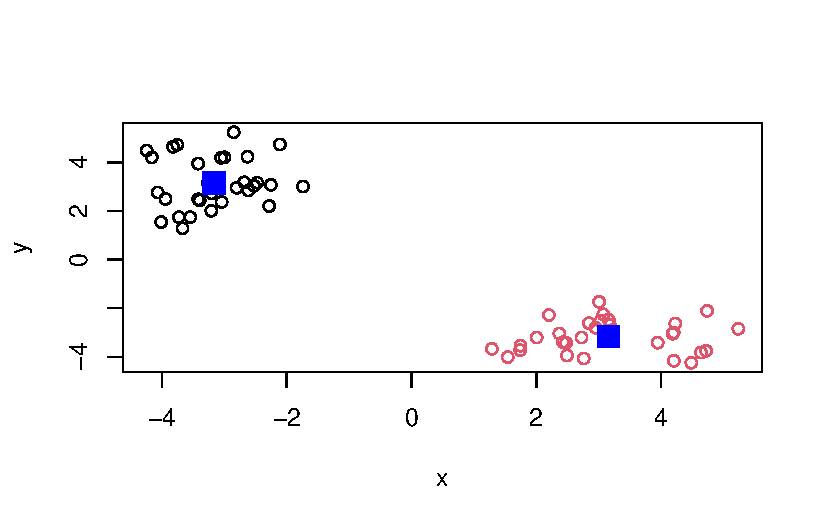
\includegraphics{Class07_files/figure-pdf/unnamed-chunk-6-1.pdf}

}

\end{figure}

\begin{quote}
Q: Let's cluster into 3 groups or same \texttt{x} data and make a plot
\end{quote}

\begin{Shaded}
\begin{Highlighting}[]
\NormalTok{km2 }\OtherTok{\textless{}{-}} \FunctionTok{kmeans}\NormalTok{(x, }\AttributeTok{centers =} \DecValTok{4}\NormalTok{)}
\FunctionTok{plot}\NormalTok{(x , }\AttributeTok{col =}\NormalTok{ km2}\SpecialCharTok{$}\NormalTok{cluster)}
\FunctionTok{points}\NormalTok{(km2}\SpecialCharTok{$}\NormalTok{centers, }\AttributeTok{col =} \StringTok{"blue"}\NormalTok{, }\AttributeTok{pch =} \DecValTok{18}\NormalTok{, }\AttributeTok{cex =} \DecValTok{2}\NormalTok{)}
\end{Highlighting}
\end{Shaded}

\begin{figure}[H]

{\centering 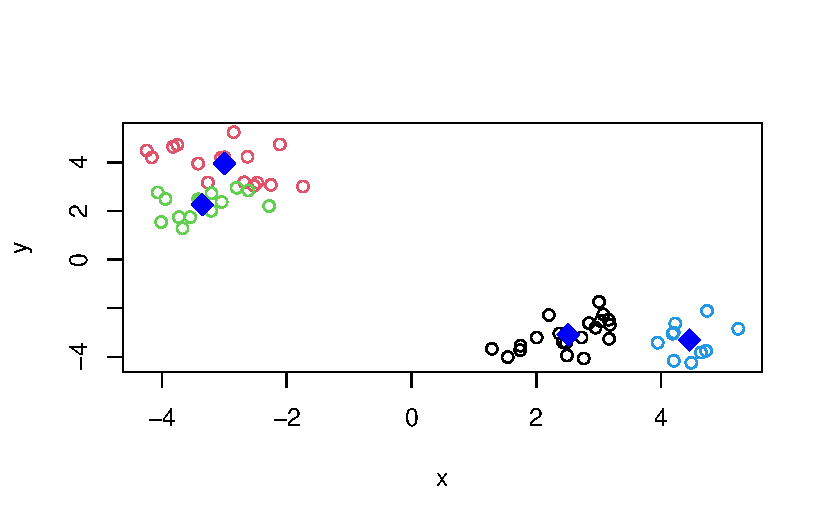
\includegraphics{Class07_files/figure-pdf/unnamed-chunk-7-1.pdf}

}

\end{figure}

\begin{Shaded}
\begin{Highlighting}[]
\CommentTok{\#totss is the measure of spread {-}{-}\textgreater{} make elbow plots, where more centers usually drops totss}
\CommentTok{\#scree plot = elbow plot, cause lower totss = better answer cause less spread (?)}
\end{Highlighting}
\end{Shaded}

\#\#Hierarchical Clustering

We can use the \texttt{hclust()} function for hierarchical clustering.
But unlike \texttt{kmeans()}, where we could pass in our data as input,
we need to give \texttt{hclust()} a ``distance matrix'' which is
produced by \texttt{dist()}. The \texttt{dist()} function gives
euclidean distance (normal distance we know for x y distances). We will
use the \texttt{dist()} function to start with

\begin{Shaded}
\begin{Highlighting}[]
\NormalTok{d }\OtherTok{\textless{}{-}} \FunctionTok{dist}\NormalTok{(x)}
\NormalTok{hc }\OtherTok{\textless{}{-}}  \FunctionTok{hclust}\NormalTok{(d)}
\NormalTok{hc}
\end{Highlighting}
\end{Shaded}

\begin{verbatim}

Call:
hclust(d = d)

Cluster method   : complete 
Distance         : euclidean 
Number of objects: 60 
\end{verbatim}

\begin{Shaded}
\begin{Highlighting}[]
\FunctionTok{plot}\NormalTok{(hc)}
\end{Highlighting}
\end{Shaded}

\begin{figure}[H]

{\centering 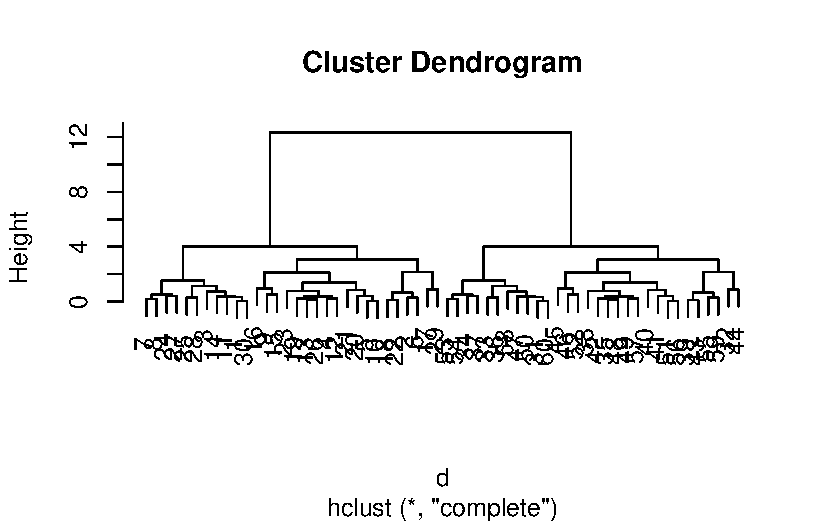
\includegraphics{Class07_files/figure-pdf/unnamed-chunk-9-1.pdf}

}

\end{figure}

I can now ``cut'' my tree with the \texttt{cutree()}to yield a cluster
membership vector.

\begin{Shaded}
\begin{Highlighting}[]
\NormalTok{grps }\OtherTok{\textless{}{-}} \FunctionTok{cutree}\NormalTok{(hc, }\AttributeTok{h =} \DecValTok{8}\NormalTok{) }\CommentTok{\#h gives height of the cut }
\NormalTok{grps}
\end{Highlighting}
\end{Shaded}

\begin{verbatim}
 [1] 1 1 1 1 1 1 1 1 1 1 1 1 1 1 1 1 1 1 1 1 1 1 1 1 1 1 1 1 1 1 2 2 2 2 2 2 2 2
[39] 2 2 2 2 2 2 2 2 2 2 2 2 2 2 2 2 2 2 2 2 2 2
\end{verbatim}

You can also tell \texttt{cutree()} to cut where it yields ``k'' number
of groups

\begin{Shaded}
\begin{Highlighting}[]
\FunctionTok{cutree}\NormalTok{(hc, }\AttributeTok{k =} \DecValTok{2}\NormalTok{)}
\end{Highlighting}
\end{Shaded}

\begin{verbatim}
 [1] 1 1 1 1 1 1 1 1 1 1 1 1 1 1 1 1 1 1 1 1 1 1 1 1 1 1 1 1 1 1 2 2 2 2 2 2 2 2
[39] 2 2 2 2 2 2 2 2 2 2 2 2 2 2 2 2 2 2 2 2 2 2
\end{verbatim}

\begin{Shaded}
\begin{Highlighting}[]
\FunctionTok{plot}\NormalTok{(x, }\AttributeTok{col =}\NormalTok{ grps )}
\end{Highlighting}
\end{Shaded}

\begin{figure}[H]

{\centering 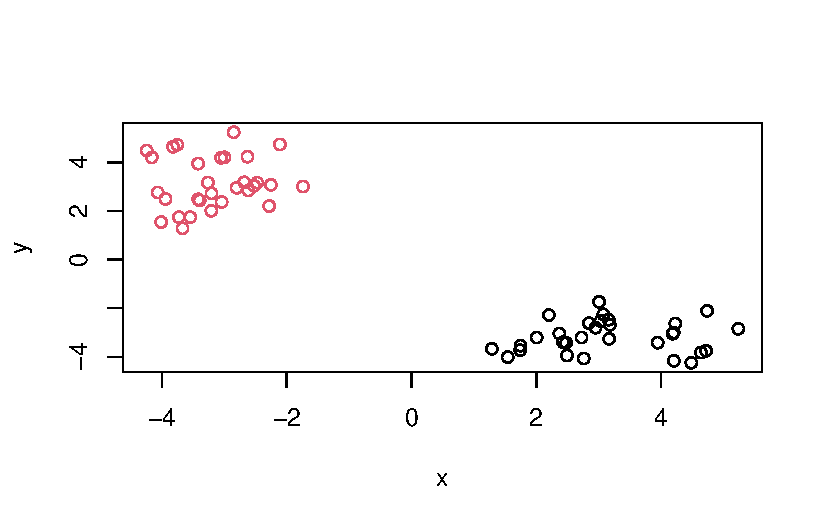
\includegraphics{Class07_files/figure-pdf/unnamed-chunk-12-1.pdf}

}

\end{figure}

\hypertarget{principal-component-analysis-pca}{%
\section{Principal Component Analysis
(PCA)}\label{principal-component-analysis-pca}}

\begin{Shaded}
\begin{Highlighting}[]
\NormalTok{url }\OtherTok{\textless{}{-}} \StringTok{"https://tinyurl.com/UK{-}foods"}
\NormalTok{y }\OtherTok{\textless{}{-}} \FunctionTok{read.csv}\NormalTok{(url) }\CommentTok{\#(url, row.names = 1)}

\FunctionTok{str}\NormalTok{(y)}
\end{Highlighting}
\end{Shaded}

\begin{verbatim}
'data.frame':   17 obs. of  5 variables:
 $ X        : chr  "Cheese" "Carcass_meat " "Other_meat " "Fish" ...
 $ England  : int  105 245 685 147 193 156 720 253 488 198 ...
 $ Wales    : int  103 227 803 160 235 175 874 265 570 203 ...
 $ Scotland : int  103 242 750 122 184 147 566 171 418 220 ...
 $ N.Ireland: int  66 267 586 93 209 139 1033 143 355 187 ...
\end{verbatim}

\begin{Shaded}
\begin{Highlighting}[]
\FunctionTok{nrow}\NormalTok{(y)}
\end{Highlighting}
\end{Shaded}

\begin{verbatim}
[1] 17
\end{verbatim}

\begin{Shaded}
\begin{Highlighting}[]
\FunctionTok{ncol}\NormalTok{(y)}
\end{Highlighting}
\end{Shaded}

\begin{verbatim}
[1] 5
\end{verbatim}

\begin{Shaded}
\begin{Highlighting}[]
\FunctionTok{dim}\NormalTok{(y)}
\end{Highlighting}
\end{Shaded}

\begin{verbatim}
[1] 17  5
\end{verbatim}

We have 17 rows and 5 columns

\begin{quote}
Q preview the first 6 rows
\end{quote}

\begin{Shaded}
\begin{Highlighting}[]
\FunctionTok{head}\NormalTok{(y)}
\end{Highlighting}
\end{Shaded}

\begin{verbatim}
               X England Wales Scotland N.Ireland
1         Cheese     105   103      103        66
2  Carcass_meat      245   227      242       267
3    Other_meat      685   803      750       586
4           Fish     147   160      122        93
5 Fats_and_oils      193   235      184       209
6         Sugars     156   175      147       139
\end{verbatim}

\#\#\#minus indexing

\begin{Shaded}
\begin{Highlighting}[]
\FunctionTok{rownames}\NormalTok{(y) }\OtherTok{\textless{}{-}}\NormalTok{ y[ , }\DecValTok{1}\NormalTok{]}
\FunctionTok{head}\NormalTok{(y)}
\end{Highlighting}
\end{Shaded}

\begin{verbatim}
                            X England Wales Scotland N.Ireland
Cheese                 Cheese     105   103      103        66
Carcass_meat    Carcass_meat      245   227      242       267
Other_meat        Other_meat      685   803      750       586
Fish                     Fish     147   160      122        93
Fats_and_oils  Fats_and_oils      193   235      184       209
Sugars                 Sugars     156   175      147       139
\end{verbatim}

\begin{Shaded}
\begin{Highlighting}[]
\NormalTok{y }\OtherTok{\textless{}{-}}\NormalTok{ y[ , }\SpecialCharTok{{-}}\DecValTok{1}\NormalTok{] }\CommentTok{\# this will remove the first column every single time you run this code (kinda bad), instead use row.names = 1 while reading the csv in to avoid this}
\FunctionTok{head}\NormalTok{(y)}
\end{Highlighting}
\end{Shaded}

\begin{verbatim}
               England Wales Scotland N.Ireland
Cheese             105   103      103        66
Carcass_meat       245   227      242       267
Other_meat         685   803      750       586
Fish               147   160      122        93
Fats_and_oils      193   235      184       209
Sugars             156   175      147       139
\end{verbatim}

\begin{Shaded}
\begin{Highlighting}[]
\FunctionTok{dim}\NormalTok{(y)}
\end{Highlighting}
\end{Shaded}

\begin{verbatim}
[1] 17  4
\end{verbatim}

\begin{quote}
Q2 Which approach to solving the `row-names problem' mentioned above do
you prefer and why? Is one approach more robust than another under
certain circumstances?
\end{quote}

I prefer the \texttt{row.names()} approach becauses I am liable to
change and rerun my code many different times and I would likely end up
with an empty dataframe.

\begin{Shaded}
\begin{Highlighting}[]
\FunctionTok{barplot}\NormalTok{(}\FunctionTok{as.matrix}\NormalTok{(y), }\AttributeTok{beside=}\NormalTok{T, }\AttributeTok{col=}\FunctionTok{rainbow}\NormalTok{(}\FunctionTok{nrow}\NormalTok{(y)))}
\end{Highlighting}
\end{Shaded}

\begin{figure}[H]

{\centering 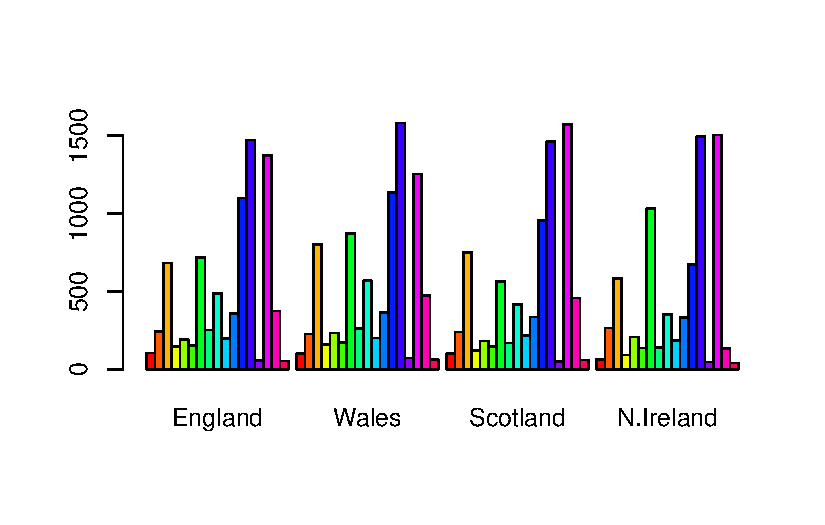
\includegraphics{Class07_files/figure-pdf/unnamed-chunk-16-1.pdf}

}

\end{figure}

\begin{quote}
Q3 Changing what optional argument in the above barplot() function
results in the following plot?
\end{quote}

\begin{Shaded}
\begin{Highlighting}[]
\FunctionTok{barplot}\NormalTok{(}\FunctionTok{as.matrix}\NormalTok{(y), }\AttributeTok{beside=}\NormalTok{F, }\AttributeTok{col=}\FunctionTok{rainbow}\NormalTok{(}\FunctionTok{nrow}\NormalTok{(y)))}
\end{Highlighting}
\end{Shaded}

\begin{figure}[H]

{\centering 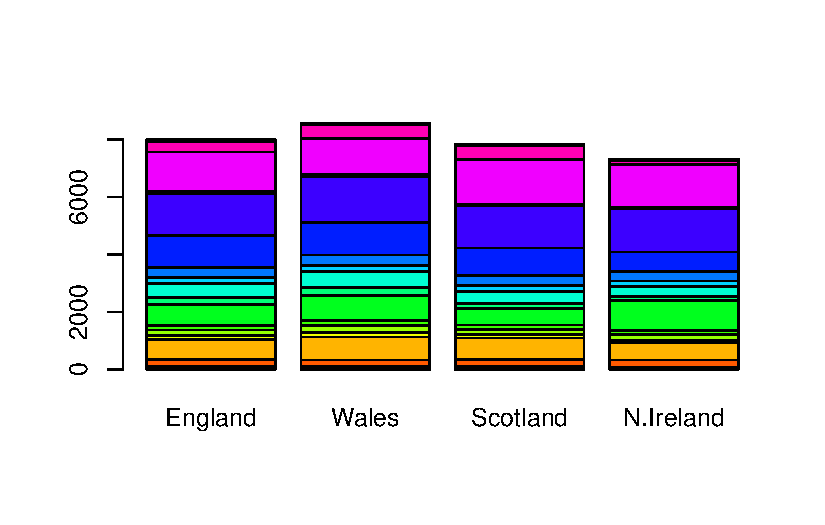
\includegraphics{Class07_files/figure-pdf/unnamed-chunk-17-1.pdf}

}

\end{figure}

Changing the beside arguement to False gives us the vertical plot.

\begin{quote}
Q5:Generating all pairwise plots may help somewhat. Can you make sense
of the following code and resulting figure? What does it mean if a given
point lies on the diagonal for a given plot?
\end{quote}

\begin{Shaded}
\begin{Highlighting}[]
\FunctionTok{pairs}\NormalTok{(y, }\AttributeTok{col =} \FunctionTok{rainbow}\NormalTok{(}\DecValTok{10}\NormalTok{), }\AttributeTok{pch =} \DecValTok{16}\NormalTok{)}
\end{Highlighting}
\end{Shaded}

\begin{figure}[H]

{\centering 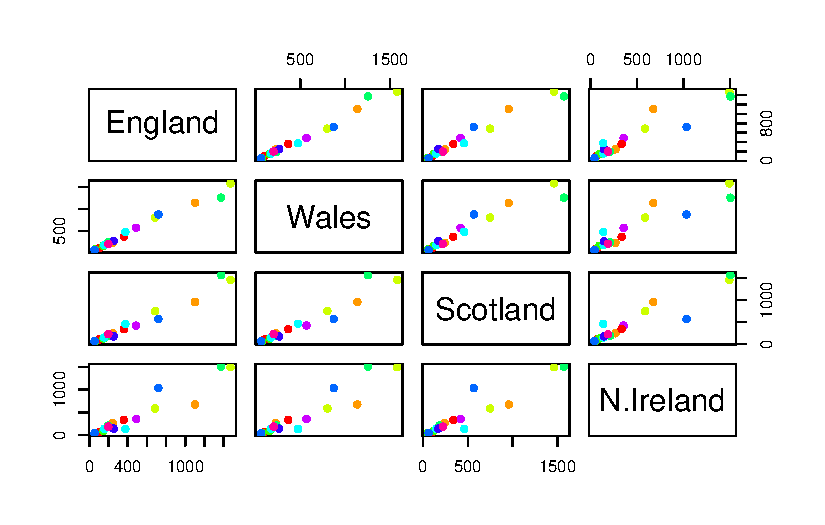
\includegraphics{Class07_files/figure-pdf/unnamed-chunk-18-1.pdf}

}

\end{figure}

\begin{Shaded}
\begin{Highlighting}[]
\CommentTok{\#reading: L{-}R = england is y axis, up{-}down = x axis if the two compared are the same, then they would be diagonal lines in that plot}
\end{Highlighting}
\end{Shaded}

\begin{quote}
Q6: What is the main differences between N. Ireland and the other
countries of the UK in terms of this data-set?
\end{quote}

The blue, orange, and cyan categories are the main differences between
N. Ireland and the other countries just from a visual standpoint.

\#\#\#using the \texttt{prcomp()} function

\begin{Shaded}
\begin{Highlighting}[]
\CommentTok{\#\textasciigrave{}t()\textasciigrave{} gives you the transposed stuff (?) idk wat do}
\NormalTok{pca }\OtherTok{\textless{}{-}}\FunctionTok{prcomp}\NormalTok{(}\FunctionTok{t}\NormalTok{(y))}
\FunctionTok{summary}\NormalTok{(pca)}
\end{Highlighting}
\end{Shaded}

\begin{verbatim}
Importance of components:
                            PC1      PC2      PC3       PC4
Standard deviation     324.1502 212.7478 73.87622 4.189e-14
Proportion of Variance   0.6744   0.2905  0.03503 0.000e+00
Cumulative Proportion    0.6744   0.9650  1.00000 1.000e+00
\end{verbatim}

\begin{Shaded}
\begin{Highlighting}[]
\FunctionTok{attributes}\NormalTok{(pca)}
\end{Highlighting}
\end{Shaded}

\begin{verbatim}
$names
[1] "sdev"     "rotation" "center"   "scale"    "x"       

$class
[1] "prcomp"
\end{verbatim}

pca\$x

\begin{quote}
Q7: Complete the code below to generate a plot of PC1 vs PC2. The second
line adds text labels over the data points.
\end{quote}

\begin{Shaded}
\begin{Highlighting}[]
\FunctionTok{plot}\NormalTok{(pca}\SpecialCharTok{$}\NormalTok{x[ ,}\DecValTok{1}\NormalTok{], pca}\SpecialCharTok{$}\NormalTok{x[ ,}\DecValTok{2}\NormalTok{], }\AttributeTok{xlab =} \StringTok{"PC1"}\NormalTok{, }\AttributeTok{ylab =} \StringTok{"PC2"}\NormalTok{, }\AttributeTok{xlim =} \FunctionTok{c}\NormalTok{(}\SpecialCharTok{{-}}\DecValTok{270}\NormalTok{, }\DecValTok{500}\NormalTok{))}
\FunctionTok{text}\NormalTok{(pca}\SpecialCharTok{$}\NormalTok{x[ ,}\DecValTok{1}\NormalTok{], pca}\SpecialCharTok{$}\NormalTok{x[ ,}\DecValTok{2}\NormalTok{], }\FunctionTok{colnames}\NormalTok{(y))}
\end{Highlighting}
\end{Shaded}

\begin{figure}[H]

{\centering 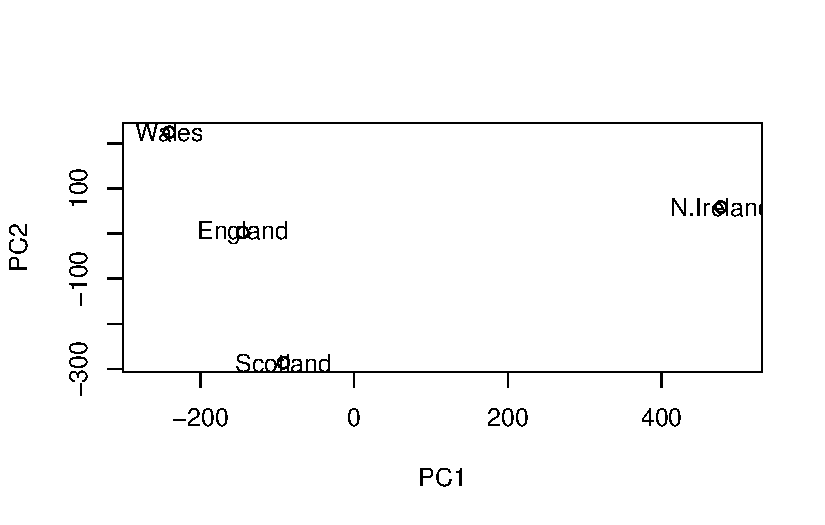
\includegraphics{Class07_files/figure-pdf/unnamed-chunk-21-1.pdf}

}

\end{figure}

\begin{quote}
Q8: Customize your plot so that the colors of the country names match
the colors in our UK and Ireland map and table at start of this
document.
\end{quote}

\begin{Shaded}
\begin{Highlighting}[]
\FunctionTok{plot}\NormalTok{(pca}\SpecialCharTok{$}\NormalTok{x[ ,}\DecValTok{1}\NormalTok{], pca}\SpecialCharTok{$}\NormalTok{x[ ,}\DecValTok{2}\NormalTok{], }\AttributeTok{xlab =} \StringTok{"PC1"}\NormalTok{, }\AttributeTok{ylab =} \StringTok{"PC2"}\NormalTok{, }\AttributeTok{xlim =} \FunctionTok{c}\NormalTok{(}\SpecialCharTok{{-}}\DecValTok{270}\NormalTok{, }\DecValTok{500}\NormalTok{))}
\FunctionTok{text}\NormalTok{(pca}\SpecialCharTok{$}\NormalTok{x[ ,}\DecValTok{1}\NormalTok{], pca}\SpecialCharTok{$}\NormalTok{x[ ,}\DecValTok{2}\NormalTok{], }\FunctionTok{colnames}\NormalTok{(y), }\AttributeTok{col =} \FunctionTok{c}\NormalTok{(}\StringTok{"red"}\NormalTok{, }\StringTok{"orange"}\NormalTok{, }\StringTok{"blue"}\NormalTok{, }\StringTok{"green"}\NormalTok{))}
\end{Highlighting}
\end{Shaded}

\begin{figure}[H]

{\centering 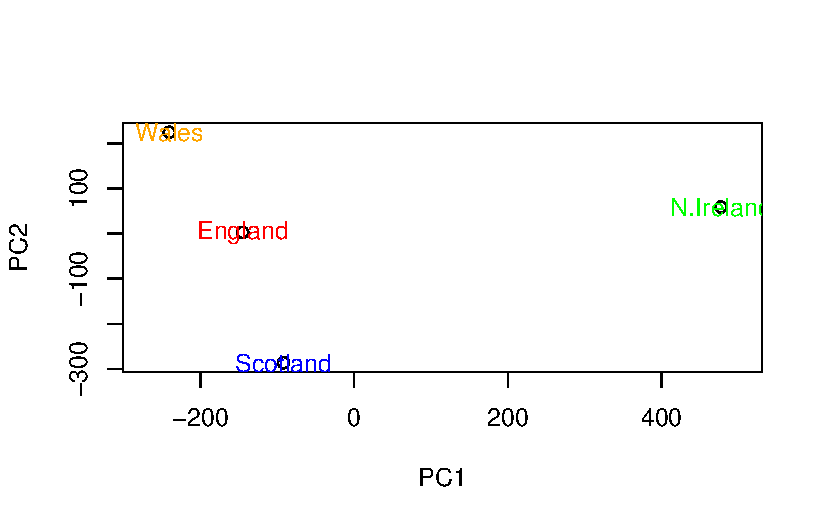
\includegraphics{Class07_files/figure-pdf/unnamed-chunk-22-1.pdf}

}

\end{figure}

\begin{quote}
Q9: Generate a similar `loadings plot' for PC2. What two food groups
feature prominantely and what does PC2 maninly tell us about?
\end{quote}



\end{document}
